\section{Introduction}
\label{sec:introduction}
The rapid progress of large language models (LLMs) has made elucidating their scaling laws a matter of central importance. These laws, which capture the intricate relationships between model architecture, parameter size, computational cost, data availability, and downstream performance~\citep{kaplan2020scaling, hoffmann2022training}, are invaluable not only because they illuminate the latent factors governing learning dynamics, but also because they provide actionable guidance on how to distribute scarce computational resources most effectively~\citep{li2025misfitting}. While extensive efforts have clarified scaling behavior, the scaling behavior of reinforcement learning (RL) post-training for LLM reasoning remains underexplored.

During pretraining, \citet{kaplan2020scaling} show that cross-entropy loss follows smooth power-law scaling in model size, dataset size, and training compute, implying that larger models trained for fewer steps are compute-optimal. \citet{hoffmann2022training} refine this by showing that, under fixed compute, scaling parameters and tokens proportionally is optimal, since many large models are undertrained. \tzl{Extending to neural-based RL, \citet{hilton2023scaling} empirically demonstrates that the intrinsic performance of convolutional neural networks (CNNs) optimized via reinforcement learning also scales like power-law with model capacity and environment interaction.}

\begin{figure*}[t] % 或者使用 [t!] / [p]
    \centering
    % --- 子图1a ---
    \begin{subfigure}[b]{0.48\textwidth}
        \centering
        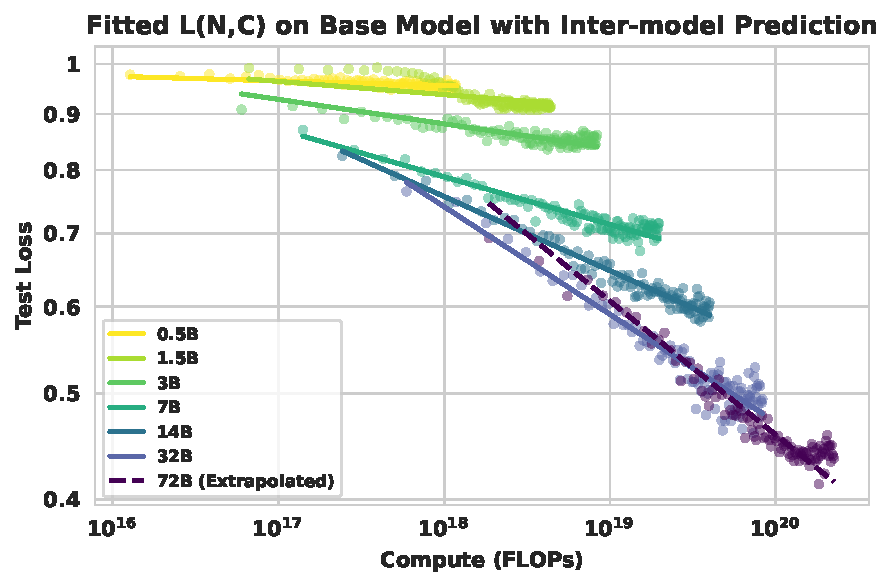
\includegraphics[width=\textwidth]{./figures/outputs/outputs/extrap_base_holdout_N_C_raw_ErrRate.pdf}
        \caption{\tzl{Inter-model Prediction for Base Model}}
        \label{fig:loss_vs_compute_exp_a}
    \end{subfigure}
    % --- 子图1b ---
    \begin{subfigure}[b]{0.49\textwidth}
        \centering
        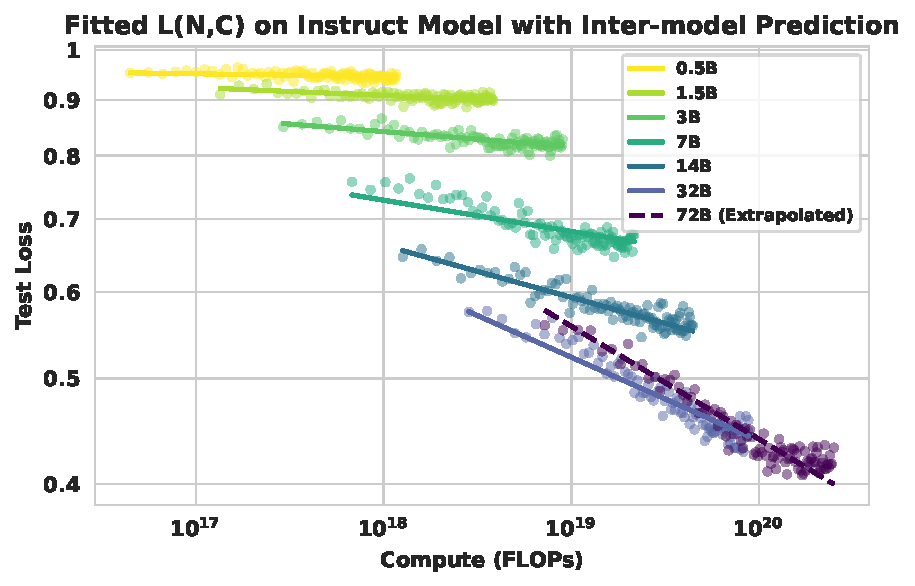
\includegraphics[width=\textwidth]{./figures/outputs/outputs/extrap_instruct_holdout_N_C_raw_ErrRate.pdf}
        \caption{\tzl{Inter-model Prediction for Instruct Model}}
        \label{fig:loss_vs_compute_exp_b}
    \end{subfigure}
\end{figure*}

\begin{figure*}[t] % 保持位置参数一致
    \ContinuedFloat % <--- 关键命令：告诉LaTeX这是上一个图的延续，不要增加图号
    \centering
    
    % --- 子图1c ---
    \begin{subfigure}[b]{0.48\textwidth}
        \centering
        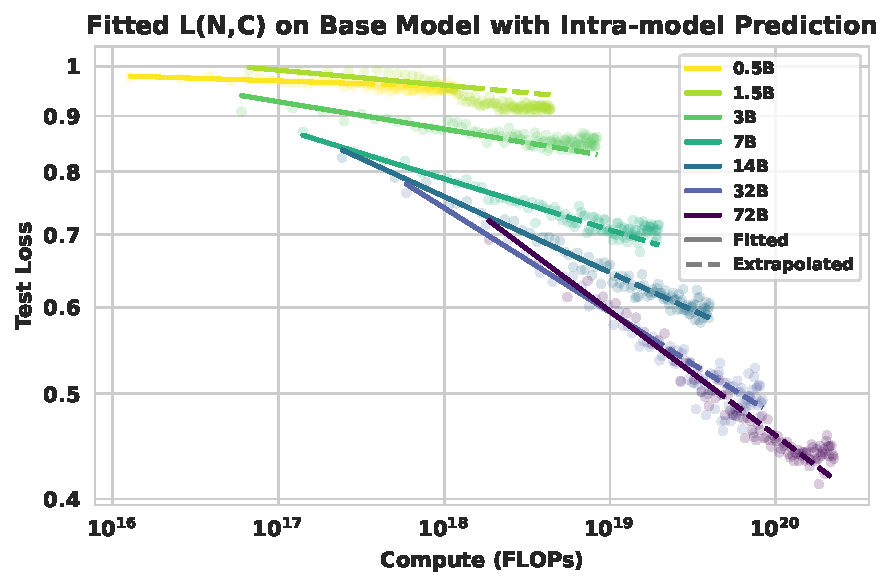
\includegraphics[width=\textwidth]{./figures/outputs/outputs/predict_base25_base_holdout_N_C_raw_ErrRate.pdf}
        \caption{\tzl{Intra-model Prediction for Base Model}}
        \label{fig:loss_vs_compute_exp_c}
    \end{subfigure}
    % --- 子图1d ---
    \begin{subfigure}[b]{0.49\textwidth}
        \centering
        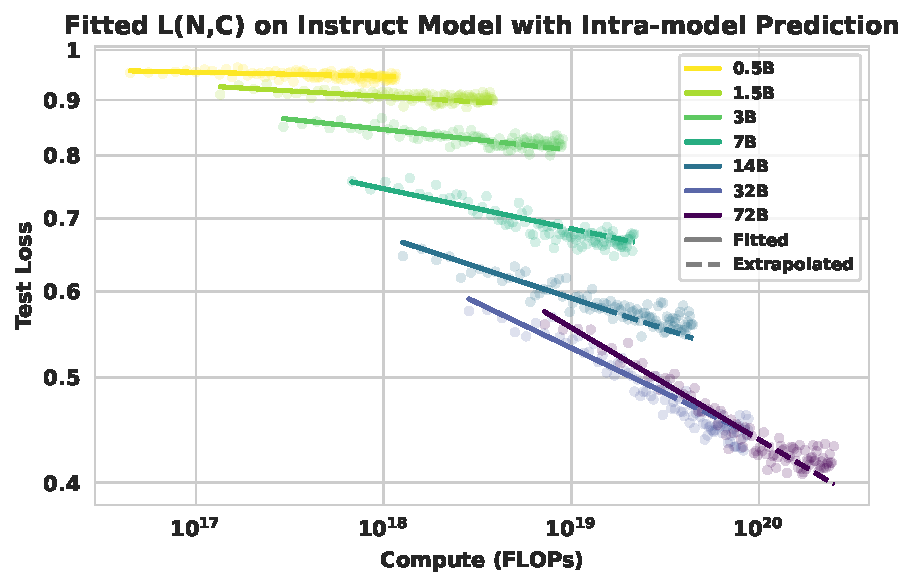
\includegraphics[width=\textwidth]{./figures/outputs/outputs/predict_instruct40_instruct_holdout_N_C_raw_ErrRate.pdf}
        \caption{\tzl{Intra-model Prediction for Instruct Model}}
        \label{fig:loss_vs_compute_exp_d}
    \end{subfigure}
    
    % 第二部分的标题，通常写 "(cont.)" 或者不写
\caption{\textbf{Empirical Scaling Behaviors in RL Post-training.} 
We validate the proposed power-law (Eq.~\ref{eq:scaling_law_intro}), which characterizes the relationship between model performance and post-training resource consumption, across models ranging from 0.5B to 72B parameters.
\textbf{(a, b) Inter-model Prediction:} Scaling coefficients fitted on smaller models (0.5B--32B) accurately predict the learning efficiency of the held-out 72B model (dashed lines) .
\textbf{(c, d) Intra-model Prediction:} The final convergence on the full dataset is extrapolated solely from early training dynamics.}
    \label{fig:intro_scaling_prediction}
    \label{fig:loss_vs_compute_exp}
\end{figure*}
While these works have established foundational scaling principles for pretraining and RL in smaller neural networks, RL has become the dominant post-training strategy for enhancing LLMs' reasoning abilities—especially in mathematics, a domain requiring long-horizon, compositional reasoning~\citep{ferrag2025llm,guo2025deepseekr1, kimi2025scaling, ahn2024large}. However, despite its growing adoption for LLM reasoning tasks, a systematic understanding of how to effectively scale RL training remains elusive. In this work, we conduct a comprehensive empirical study to characterize these scaling behaviors across three critical resource regimes: (1) the \textbf{compute-constrained} scenario, where we determine the optimal model size to minimize test loss (\textbf{$1-PassRate$}) under a fixed FLOPs budget; (2) the \textbf{data-constrained} scenario, where we identify the model size yielding the lowest test loss with limited unique samples; and (3) the \textbf{data reuse} scenario, where we explore the trade-off between data uniqueness and reuse intensity under a fixed total data volume.


Based on our analysis across these regimes, we propose a \textbf{predictive formulation} that characterizes the relationship between test loss $L$, model size $N$, and resource budget $X$ (where $X$ denotes either Compute $C$ or Data $D$). We find that the scaling behavior can be effectively modeled by a power-law that exhibits a log-linear relationship between test loss and resource budget:
\begin{equation}
    \label{eq:scaling_law_intro}
    \log L(N, X) = -k(N) \cdot \log X + E(N)
\end{equation}
Here, $k(N)$ represents the learning efficiency, which our empirical results show does not grow indefinitely with increasing model scale. Instead, it follows a saturation trend modeled by:
\begin{equation}
    \label{eq:efficiency_intro}
    k(N) = \frac{K_{\text{max}}}{1 + \frac{N_{0}}{N}}
\end{equation}
This formulation (Eq.~\ref{eq:efficiency_intro}) shows that: while larger models consistently exhibit higher learning efficiency, the marginal gains in efficiency diminish as model size increases, asymptotically approaching a theoretical limit $K_{\text{max}}$.

To empirically validate this law and determine its parameters, \tzl{we fine-tune 63 LLMs with reinforcement learning on over 50k mathematics problems}, based on the Qwen2.5 model family~\citep{qwen2025qwen25technicalreport}. Figure~\ref{fig:loss_vs_compute_exp} shows that, \tzl{within the 0.5B-72B range}, the loss reduction brought by RL follows an approximately log-linear trend with compute. Importantly, larger models not only have better initial performance but also generally have more efficiency in computation and data utilization during the optimization process. Further analysis confirms that our proposed formulation (Eq.~\ref{eq:scaling_law_intro}) exhibits notable predictability, while also verifying the saturation effect in efficiency gains.

We additionally analyze the data-constrained regime, where we demonstrate that data reuse is a highly effective strategy. We validate the generality of our findings through extensive ablation studies on both base and instruct model series. Besides, we have also conducted experiments to study the impact of the rollout number in the GRPO algorithm~\citep{shao2024deepseekmathpushinglimitsmathematical}, shown in Appendix~\ref{subsec:ablation_grpo}. These investigations establish fundamental scaling relationships for RL post-training, providing a quantitative foundation and practical guidelines for resource-efficient model refinement.

Specifically, our key findings can be summarized as follows:
\vskip -0.2in
\begin{itemize}
    \item \textbf{We propose a predictive power-law formulation for RL post-training}, which models the scaling relationship between test loss, model size, compute, and data. This formulation enables reliable prediction of both larger model performance and late-stage training trajectories.
    \item Larger models consistently exhibit superior compute and data efficiency in the RL post-training, but \textbf{the marginal gains in efficiency diminish gradually with increasing model scale}, revealing an inherent saturation trend.
    \item In data-limited settings, repeated exposure to a small dataset is nearly as effective as using larger corpora, \textbf{highlighting data reuse as a practical strategy}.
\end{itemize}
